\section{Energy Estimator Graphs}\label{sec::energyEst}
\begin{figure}[H]
	\begin{minipage}[t]{0.45\linewidth}
		\begin{center}
            \label{fig::amp1}
			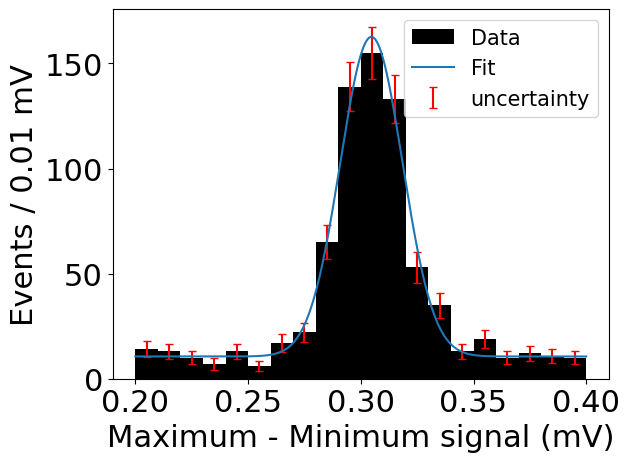
\includegraphics[width=\textwidth]{figures/amp1.png}
			\caption{
                $10\unit{KeV}$ calibration particle detection events, grouped by pre-calibration energy estimate, overlaid with Gaussian best fit.\\
                \textbf{Energy Estimate}: Max - Min detected signal ($\unit{mV}$).
            }
		\end{center}
	\end{minipage}
    \hfill
	\begin{minipage}[t]{0.45\linewidth}
		\begin{center}
            \label{fig::amp1--cal}
			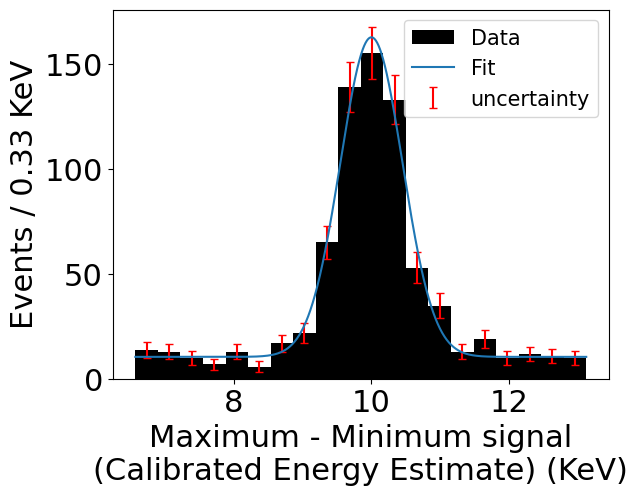
\includegraphics[width=\textwidth]{figures/amp1--calibrated.png}
			\caption{
                $10\unit{KeV}$ calibration particle detection events, grouped by calibrated energy estimate, overlaid with Gaussian best fit. x-axis has been proportionally calibrated to place Gaussian fit mean at $10\unit{KeV}$ \\
                \textbf{Energy Estimate}: Max - Min detected signal ($\unit{mV}$).
            }
		\end{center}
	\end{minipage}
\end{figure}

\begin{figure}[H]
	\begin{minipage}[t]{0.45\linewidth}
		\begin{center}
            \label{fig::amp2}
			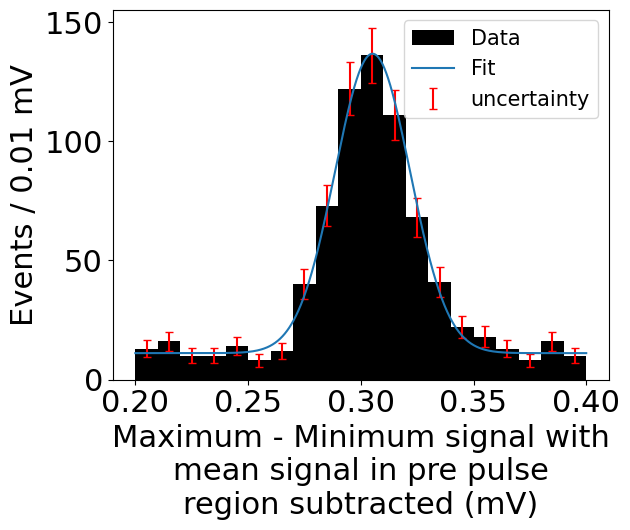
\includegraphics[width=\textwidth]{figures/amp2.png}
			\caption{
                $10\unit{KeV}$ calibration particle detection events, grouped by pre-calibration energy estimate, overlaid with Gaussian best fit.\\
                \textbf{Energy Estimate}: Max detected signal minus mean pre pulse signal  ($\unit{mV}$)
            }
		\end{center}
	\end{minipage}
    \hfill
	\begin{minipage}[t]{0.45\linewidth}
		\begin{center}
            \label{fig::amp2--cal}
			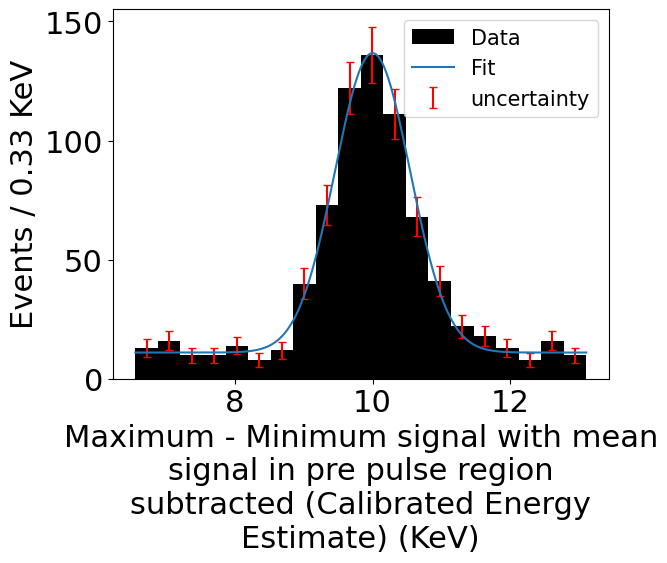
\includegraphics[width=\textwidth]{figures/amp2--calibrated.png}
			\caption{
                $10\unit{KeV}$ calibration particle detection events, grouped by calibrated energy estimate, overlaid with Gaussian best fit. x-axis has been proportionally calibrated to place Gaussian fit mean at $10\unit{KeV}$ \\
                \textbf{Energy Estimate}: Max detected signal ($\unit{mV}$) minus mean pre pulse signal
            }
		\end{center}
	\end{minipage}
\end{figure}
\begin{figure}[H]
	\begin{minipage}[t]{0.45\linewidth}
		\begin{center}
            \label{fig::area1}
			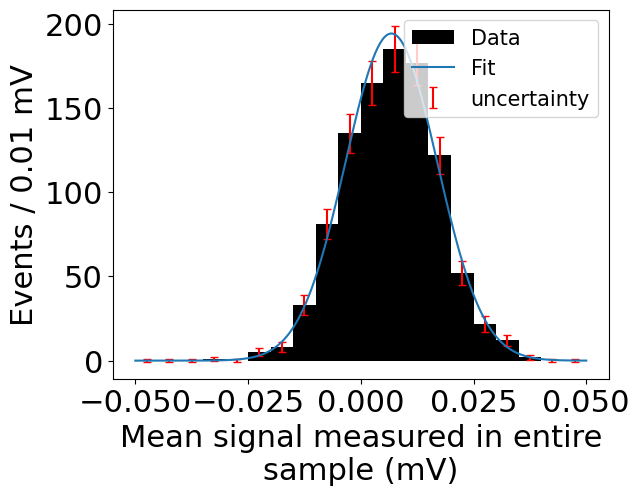
\includegraphics[width=\textwidth]{figures/area1.png}
			\caption{
                $10\unit{KeV}$ calibration particle detection events, grouped by pre-calibration energy estimate, overlaid with Gaussian best fit.\\
                \textbf{Energy Estimate}: Mean detected signal ($\unit{mV}$)
            }
		\end{center}
	\end{minipage}
    \hfill
	\begin{minipage}[t]{0.45\linewidth}
		\begin{center}
            \label{fig::area1--cal}
			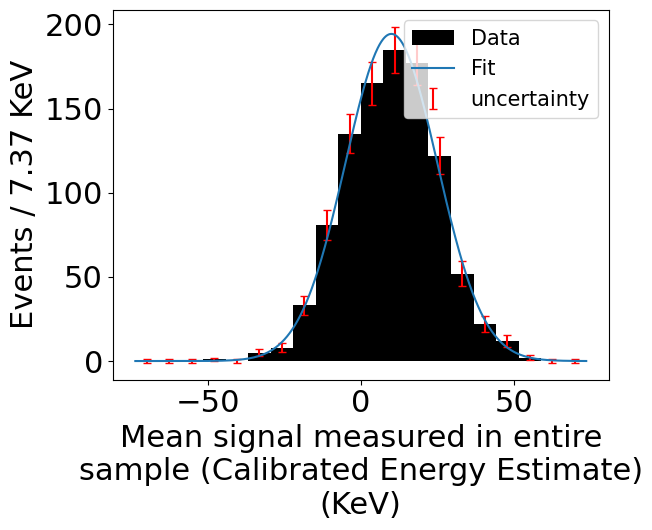
\includegraphics[width=\textwidth]{figures/area1--calibrated.png}
			\caption{
                $10\unit{KeV}$ calibration particle detection events, grouped by calibrated energy estimate, overlaid with Gaussian best fit. x-axis has been proportionally calibrated to place Gaussian fit mean at $10\unit{KeV}$ \\
                \textbf{Energy Estimate}: Mean detected signal ($\unit{mV}$)
            }
		\end{center}
	\end{minipage}
\end{figure}

\begin{figure}[H]
	\begin{minipage}[t]{0.45\linewidth}
		\begin{center}
            \label{fig::area2}
			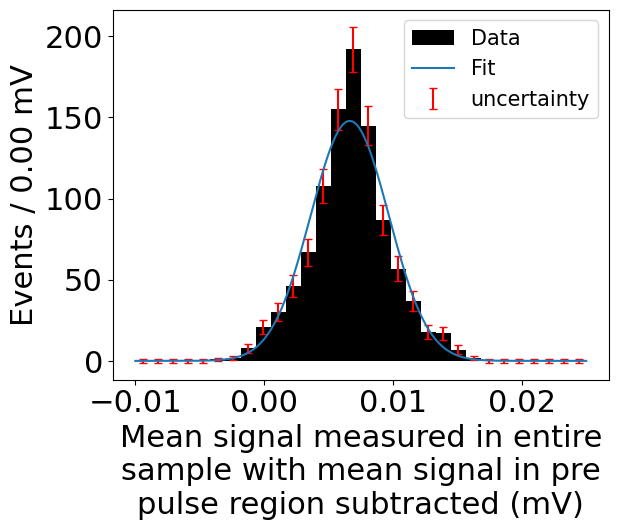
\includegraphics[width=\textwidth]{figures/area2.png}
			\caption{
                $10\unit{KeV}$ calibration particle detection events, grouped by pre-calibration energy estimate, overlaid with Gaussian best fit.\\
                \textbf{Energy Estimate}: Mean detected signal minus mean pre pulse signal  ($\unit{mV}$)
            }
		\end{center}
	\end{minipage}
    \hfill
	\begin{minipage}[t]{0.45\linewidth}
		\begin{center}
            \label{fig::area2--cal}
			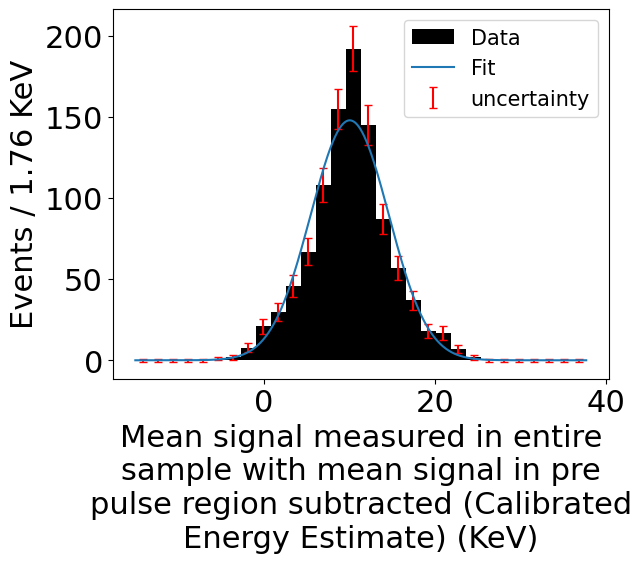
\includegraphics[width=\textwidth]{figures/area2--calibrated.png}
			\caption{
                $10\unit{KeV}$ calibration particle detection events, grouped by calibrated energy estimate, overlaid with Gaussian best fit. x-axis has been proportionally calibrated to place Gaussian fit mean at $10\unit{KeV}$ \\
                \textbf{Energy Estimate}: Mean detected signal minus mean pre pulse signal  ($\unit{mV}$)
            }
		\end{center}
	\end{minipage}
\end{figure}


\begin{figure}[H]
	\begin{minipage}[t]{0.45\linewidth}
		\begin{center}
            \label{fig::area3}
			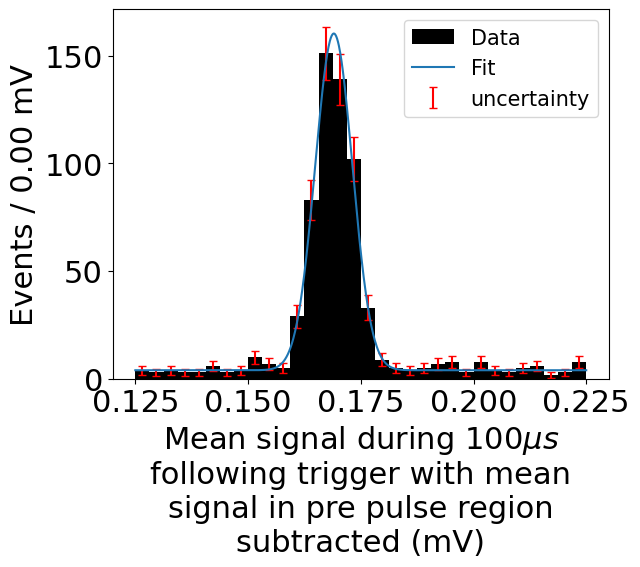
\includegraphics[width=\textwidth]{figures/area3.png}
			\caption{
                $10\unit{KeV}$ calibration particle detection events, grouped by pre-calibration energy estimate, overlaid with Gaussian best fit.\\
                \textbf{Energy Estimate}: Mean detected signal in the $100\unit{\micro s}$ after pulse start minus mean pre pulse signal  ($\unit{mV}$)
            }
		\end{center}
	\end{minipage}
    \hfill
	\begin{minipage}[t]{0.45\linewidth}
		\begin{center}
            \label{fig::area3--cal}
			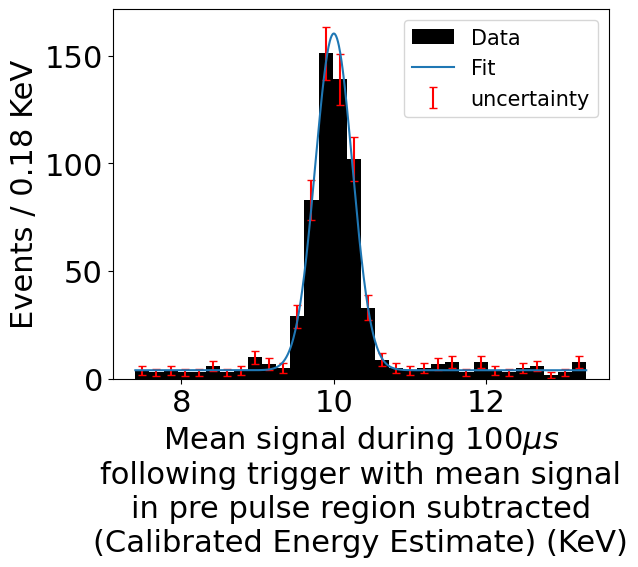
\includegraphics[width=\textwidth]{figures/area3--calibrated.png}
			\caption{
                $10\unit{KeV}$ calibration particle detection events, grouped by calibrated energy estimate, overlaid with Gaussian best fit. x-axis has been proportionally calibrated to place Gaussian fit mean at $10\unit{KeV}$ \\
                \textbf{Energy Estimate}: Mean detected signal in the $100\unit{\micro s}$ after pulse start minus mean pre pulse signal  ($\unit{mV}$)
            }
		\end{center}
	\end{minipage}
\end{figure}
\begin{figure}[H]
	\begin{minipage}[t]{0.45\linewidth}
		\begin{center}
            \label{fig::pulseFit}
			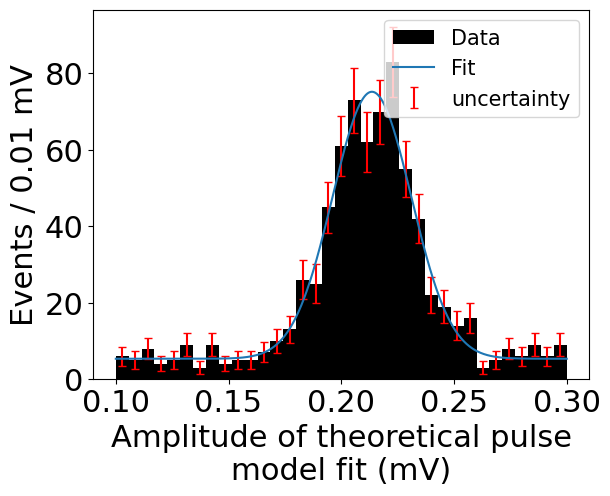
\includegraphics[width=\textwidth]{figures/pulseFit.png}
			\caption{
                $10\unit{KeV}$ calibration particle detection events, grouped by pre-calibration energy estimate, overlaid with Gaussian best fit.\\
                \textbf{Energy Estimate}: Amplitude of theoretical pulse model fit (mV)
            }
		\end{center}
	\end{minipage}
    \hfill
	\begin{minipage}[t]{0.45\linewidth}
		\begin{center}
            \label{fig::pulseFit--cal}
			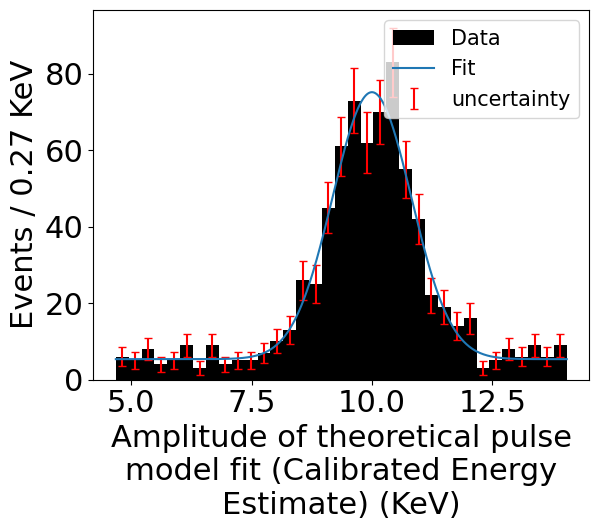
\includegraphics[width=\textwidth]{figures/pulseFit--calibrated.png}
			\caption{
                $10\unit{KeV}$ calibration particle detection events, grouped by calibrated energy estimate, overlaid with Gaussian best fit. x-axis has been proportionally calibrated to place Gaussian fit mean at $10\unit{KeV}$ \\
                \textbf{Energy Estimate}: Amplitude of theoretical pulse model fit (mV)
            }
		\end{center}
	\end{minipage}
\end{figure}
